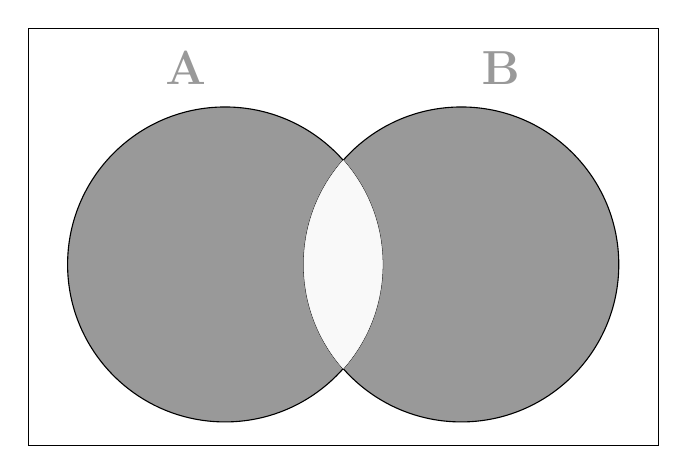
\begin{tikzpicture}
\begin{scope}[fill opacity=.4]
\draw (-4, 4) rectangle (4, -1.3);
\draw[fill=black, draw=black] 
(-1.5, 1) circle (2);
\draw[fill=black, draw=black] 
(1.5, 1) circle (2);
\node at (-2, 3.5) {\LARGE\textbf{A}};
\node at (2, 3.5) {\LARGE\textbf{B}};
\begin{scope}
\clip (-1.5, 1) circle (2);
\clip (1.5, 1) circle (2);
\draw[fill=white, draw=black] 
(-5, 4.5) rectangle (5, -2);
\draw[fill=white, draw=black] 
(-5, 4.5) rectangle (5, -2);
\draw[fill=white, draw=black] 
(-5, 4.5) rectangle (5, -2);
\draw[fill=white, draw=black] 
(-5, 4.5) rectangle (5, -2);
\draw[fill=white, draw=black] 
(-5, 4.5) rectangle (5, -2);
\draw[fill=white, draw=black] 
(-5, 4.5) rectangle (5, -2);
\draw[fill=white, draw=black] 
(-5, 4.5) rectangle (5, -2);
\end{scope}
\end{scope}
\end{tikzpicture}
